%automated figure captioning

\chapter{Theory}


An overview of the relevant theoretical concepts is included in this chapter. Key terms are defined, including how they are anchored within the research. Relevant theoretical concepts include citizen science, stakeholders, local knowledge, vulnerability, place, and awareness. Resilience is further conceptualised and is considered as the outcome of interacting systems: natural systems, technological systems and social systems. By expanding upon \cite{cutter_place-based_2008} and \cite{cutter_community_2020} to answer the needs highlighted by \cite{rasanen_conceptualizing_2020}, projected resilience of place is suggested as the theoretical framework.

\section{Key Terms}


\subsection{Citizen Science}
Citizen science can take a variety of forms, but the common factor is the involvement of volunteers: people who chose to use their time to assist in science who are not paid for this time (\cite{pocock_choosing_2014}). Considering \cite{tweddle_guide_2012} (Guide to citizen science: developing, implementing and evaluating citizen science to study biodiversity and the environment in the UK) , the participation of volunteers is deemed critical for this project: the data required would not be accessible using other techniques (\cite{tweddle_guide_2012}). Furthermore, it may improve the volunteers' awareness of SLEs in Trondheim (\cite{gerkensmeier_governing_2018}).  The volunteers contributions were respected and the impact on their time was minimised. Going forward, the citizen science volunteers will be referred to as subjects. 

\subsection{Stakeholders}
The stakeholders primarily considered during this project are the people who live, commute or work in coastal Trondheim. . Other stakeholders considered are people with attachment to the research sites as well as well as planners and policy makers. These were chosen following \cite{reed_stakeholder_2008} work on stakeholder analysis which reviewed different approaches and suggests that stakeholder analysis must be viewed as a participatory process which requires the integration of local knowledge and trust. As stated in the Methodology (section \ref{data-collection}) targeting of potential subjects utilising the decided upon stakeholders was carried out. 


\subsection{Local Knowledge}

Local knowledge is considered here as place-based competence, information and resources (\cite{setten_we_2019}). Over time,  local knowledge is co-produced and maintained by a range of experts both locally situated and beyond the place's boundaries: "We draw on what we know anyway" is a very succinct conceptualisation of local knowledge within the context of disaster risk management (\cite{setten_we_2019}). 

\begin{figure}[ht]
    \centering
    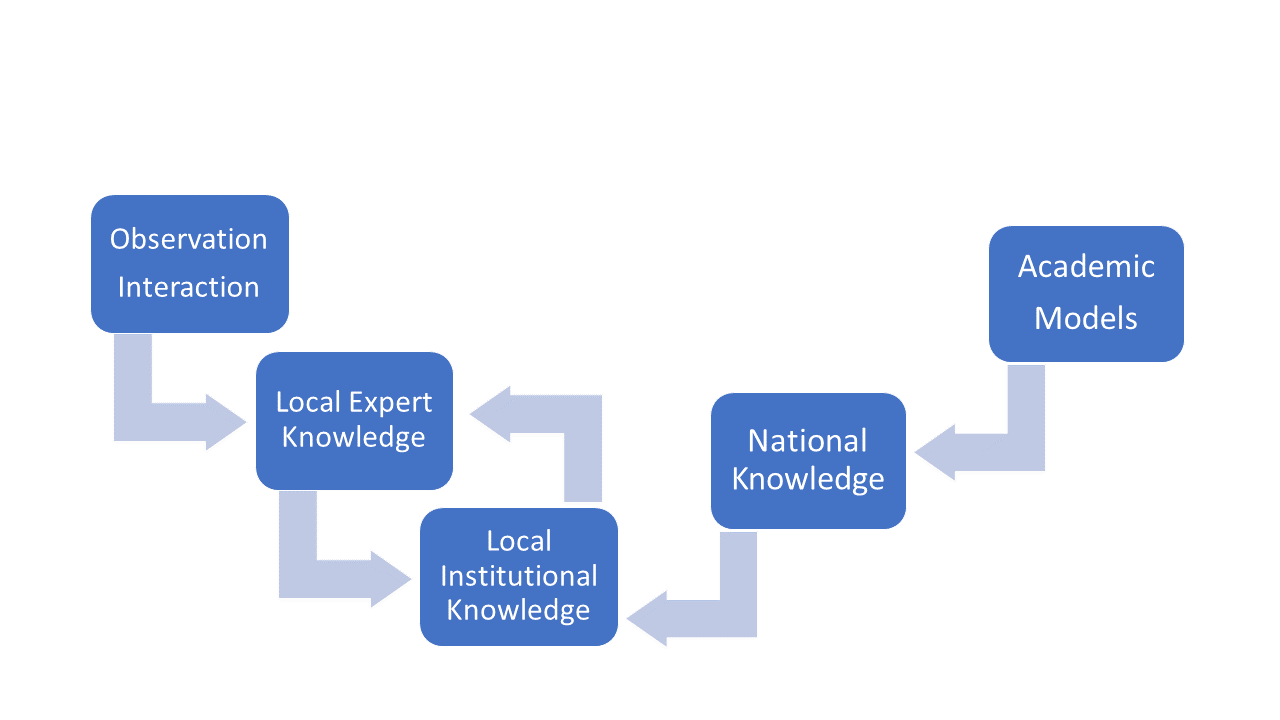
\includegraphics[width=1\textwidth]{fig_theory/local knowledge accumulation.png}
    \caption{Production of Local Knowledge }{ Local expert knowledge is produced by observation and interactions, often in the local sphere. Local expert knowledge co-produces with local institutional knowledge, each feeding into the other. Academic models help produce national knowledge which in turn feeds into local institutional knowledge.Figure created using Microsoft PowerPoint using the information stream outlined in \cite{setten_we_2019} and \cite{rod_integrated_2012}.}
    \label{fig:local_knowledge}
\end{figure}


Figure ~\ref{fig:local_knowledge} shows Local expert knowledge is created from local observations and local interactions. Yet, local expert knowledge is also created from local institutional knowledge. This local institutional knowledge is in turn co-produced by local expert knowledge. In this case, the local expert knowledge is often considered more informal than the formalised local institutional knowledge, but does not need to be limited to this. An example of informal local expert knowledge co-producing local institutional knowledge is that sjøbadet members (swimming club and outdoor facility situated in Brattøra (figure \ref{fig:research_site}) noticed that they need to remove some of their decking in winter to prevent it getting get damaged in winter storms, this information is spread during casual conversation by their members and later written on their noticeboard making it more formalised institutional knowledge. 
\paragraph{}

Academic models and national knowledge do feed into local institutional knowledge and this in turn feeds into local expert knowledge. For example all members of Trondheim Kajakk Klubb are taught the safest way to paddle from the marina in Skansen (figure \ref{fig:research_site}) to the Island of Munkholmen. This information is based both on individuals previous experience and on Norgeskart, nationally available maps which include the ferry route (\cite{kartverket_norgeskart_2023}). 

\paragraph{}
Considering disaster risk management, the local institutional and expert knowledge does not always feed back to these other producers of knowledge (\cite{rod_integrated_2012}). The questions about the alignment between local knowledge and academic models of the changing SLEs influenced the creation of this project. Increasing the interplay between local expert knowledge and local institutional knowledge can increase resilience (\cite{setten_we_2019}).

\paragraph{}

Local knowledge is often highlighted as a key facet of community resilience (\cite{setten_we_2019}). The assumption is that higher levels of local knowledge, particularly higher levels of awareness about natural systems and natural hazards, increases community resilience.  How local knowledge interacts with community resilience and where this belongs in a place-based conceptualisation of resilience is discussed in the social systems of resilience section below. Awareness of local risk is here considered as a facet of local knowledge.  


 
\subsection{Vulnerability}
Vulnerability of place is affected by both biophysical and social factors, including local knowledge (\cite{opach_seeking_2020}). Potential exposure to hazards, combined with coping ability, is the broad conceptualisation of vulnerability of place as used here (\cite{rygel_method_2006}). Potential exposure to hazards can be considered as the predisposition of a place to be negatively affected by an event (\cite{lujala_quantifying_2014}). Physical vulnerability is a places characteristics which influence its capacity to be impacted by SLEs. According to \cite{rod_integrated_2012}, vulnerability cannot be directly measured and as such an observable characteristic is needed.  As stated in methodology (section \ref{data-collection}) the observable characteristic used to determine physical vulnerability is the ability to be flooded due to SLEs, determined from direct observation of the research sites combined with models from \cite{kartverket_se_2020} and planning documents. The determination of vulnerability and resilience within this paper is focused on a single hazard, rather than multi-hazard. The strengths and limitations of this technique are discussed later. 
\paragraph{}
This research does not aim to create new vulnerability indices, but does recognise their usefulness. Vulnerability indices are an attempt to measure the potential exposure to hazards combined with the coping ability, but usually splits these into biophysical vulnerability  and social vulnerability (\cite{rod_integrated_2012}). The literature often labels biophysical vulnerability as exposure and social vulnerability as capacity (\cite{rod_integrated_2012}). There is ongoing debate about whether it is appropriate to split the analysis of biophysical and social vulnerability (\cite{lujala_quantifying_2014}). Here, the conceptualisation of resilience includes the factors of biophysical and social vulnerability within a dynamic process, rather than as a static value.

\subsection{Place and Space-time} 
To understand resilience, we must ask for whom; of what; to what; of where; how and when (\cite{cutter_community_2020}), (\cite{moser_turbulent_2019}). Resilience is temporally and spatially dynamic (\cite{cutter_community_2020}). Hence, a short description of what is meant here by space, time and place is necessary. The conceptualisation used here is inline with \cite{massey_for_2005}, where space is the dimension of simultaneity and is part of space-time. In this view, space is considered as the dimension of things being and, importantly, occurring at the same time. In contrast, time is considered as things occurring one after the other. This conceptualisation of space-time is relevant for private, public and even virtual spaces and gives room for the social networks that operate within these spaces (\cite{massey_for_2005}; \cite{allen_rethinking_1998}; \cite{del_casino_social_2009}).

\paragraph{}
The four chosen research places are created upon a combination of public and private space. The majority of the edge of the water in Norway can be considered public space, but there is also space allocated to specific groups which can create feelings of in-place versus out-of-place. Place is considered as an assemblage of traces. These traces range from the historical and global to the local and present and it is these combinations of traces which combine to make these places (\cite{anderson_understanding_2015}; \cite{massey_for_2005}). As well as explicit group membership, the traces of place influence who can feel in-place and what is culturally and legally allowable uses of the place (\cite{anderson_understanding_2015}). The four research sites include a wide demographic of users who can be considered in-place, but the power relationships and the in-place members affect the resilience of the location. 

\subsection{Awareness}
To understand the present resilience of a place requires an understanding of the awareness of the people who interact with and define the place. An individual’s ability to rank their level of awareness about a subject is a long investigated and debated topic. It is generally preferable to allow them to display their level of awareness rather than ask them on a sliding scale how aware they are. This is especially important when trying to explore knowledge which may have previously been seen as lesser.

\paragraph{}
Figure ~\ref{fig:hazard_to_behaviour} shows the Natural Hazard Risk to Behaviour Pipeline drawing from the work of \cite{whitmarsh_are_2008} and \cite{lujala_climate_2015}. Awareness of natural hazard risk is influenced by information sources an individual consumes. This information is filtered through the prisms of perceived distance from the risk, personal experience of prior and similar risks and the individual's values such as trust in the information source or personal beliefs. This creates the individual's attitude to the natural hazard risk. This attitude combined with the resources at their disposal influences the individuals behaviour.

\paragraph{}


\begin{figure}[h]
    \centering
    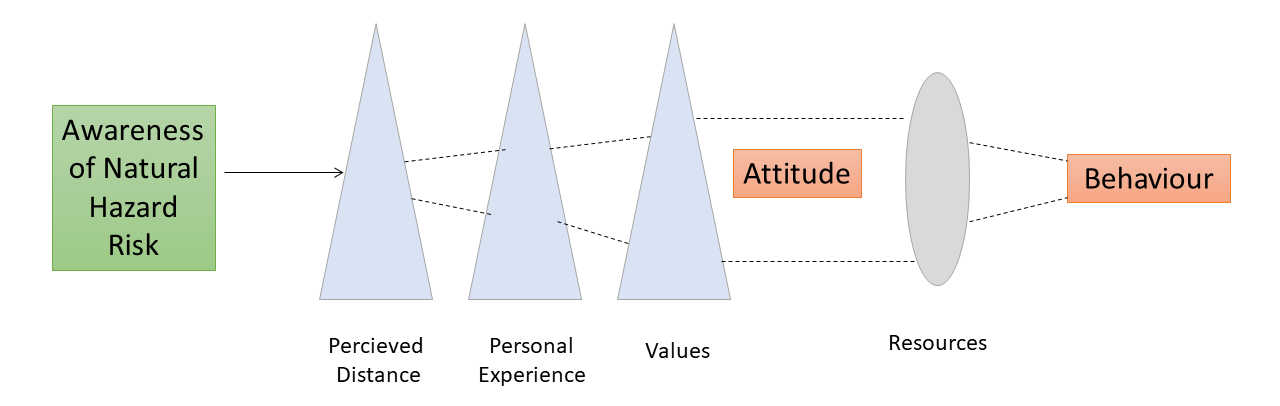
\includegraphics[width=1\textwidth]{fig_theory/new_awareness_ lujala_whitmarsh.png}
     \caption{Awareness of Natural Hazard Risk to Behaviour Pipeline}{ drawing from \cite{lujala_climate_2015} and \cite{whitmarsh_are_2008}, created using Inkscape.  The awareness of Natural Hazard risk is the awareness of the individual about the risk. This is filtered through the three prisms of perceived distance, then personal experience and then values which have significant impact on how the information of natural hazard risk is manifested as attitude.  
    This attitude to the information about natural hazard risk is then filtered through the lens of resources before influencing the behaviour of the individual.} 
    \label{fig:hazard_to_behaviour}
\end{figure} 
\paragraph{}
This is a simplified model of an individual's thought process, but it can be helpful when predicting behaviour. There is an assumptions that those with higher levels of awareness about risks are more likely to have certain attitudes and in turn certain behaviours, but this is not always the case (\cite{lujala_climate_2015}).  Awareness of the changing tides and risk of storm surges is considered here as an aspect of local knowledge and is one of the key factors investigated to determine the resilience of Trondheim to SLEs. 

\section{Systems of Resilience }

\subsection{Social Systems Impacting Resilience}
Community resilience is considered here as a key aspect of social systems, rather than as a distinct concept. Local knowledge is considered as conceptually part of community resilience. The hierarchy of these concepts is shown in figure ~\ref{fig:social_resilience}. An understanding of people's awareness of a risk is key to determining the social system resilience to that risk. This can be considered as part of social vulnerability.

\begin{figure}[h]
    \centering
    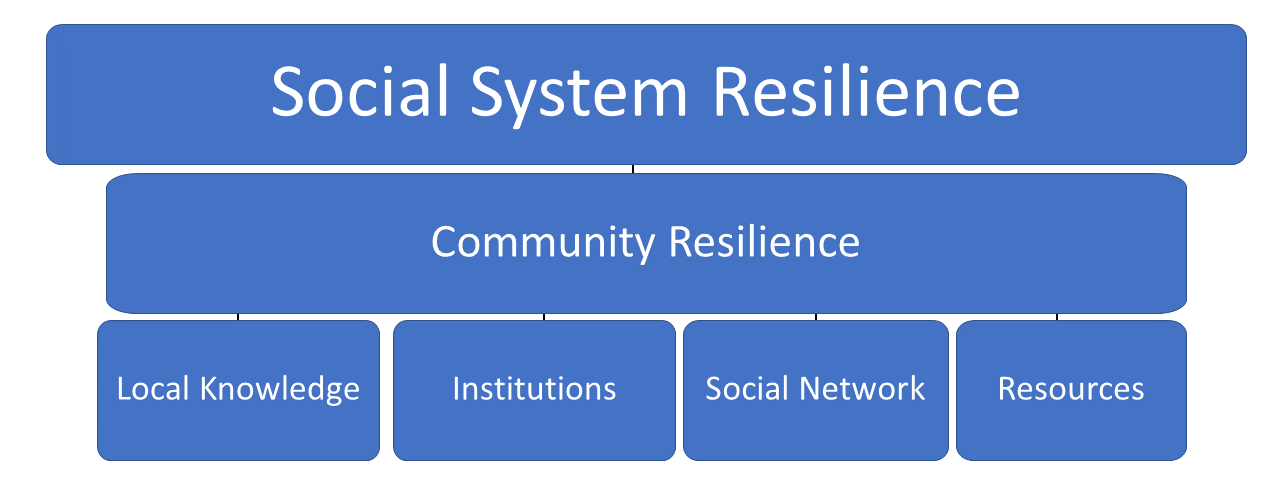
\includegraphics[width=1\textwidth]{fig_theory/new_social_system.png}
    \caption{Relationship between Community Resilience and Social System Resilience}{. Resources, social network, institutions and local knowledge are all important factors of Community Resilience. Within this text, community resilience is considered as a major facet of social system resilience. Social system resilience is the overarching idea which is situated above community resilience.}
    \label{fig:social_resilience}
\end{figure}
\paragraph{}

A place's resources, social network, institutions and local knowledge are key factors determining its community resilience. This in turn is key in the determination of social system resilience, but social system resilience is a wider conceptualisation that community resilience, though there are strong similarities (\cite{cutter_community_2020}). The conceptualisation of social system resilience is particularly important where place-based understanding of community is dominant, such as in Norway (\cite{rasanen_conceptualizing_2020}). Norway also has a specific hierarchy of responsibility for disaster risk management, which strongly impacts the social system resilience of places within the country, as outlined, in figure ~\ref{fig:drm_responsibility}.


\begin{figure} [h]
    \centering
    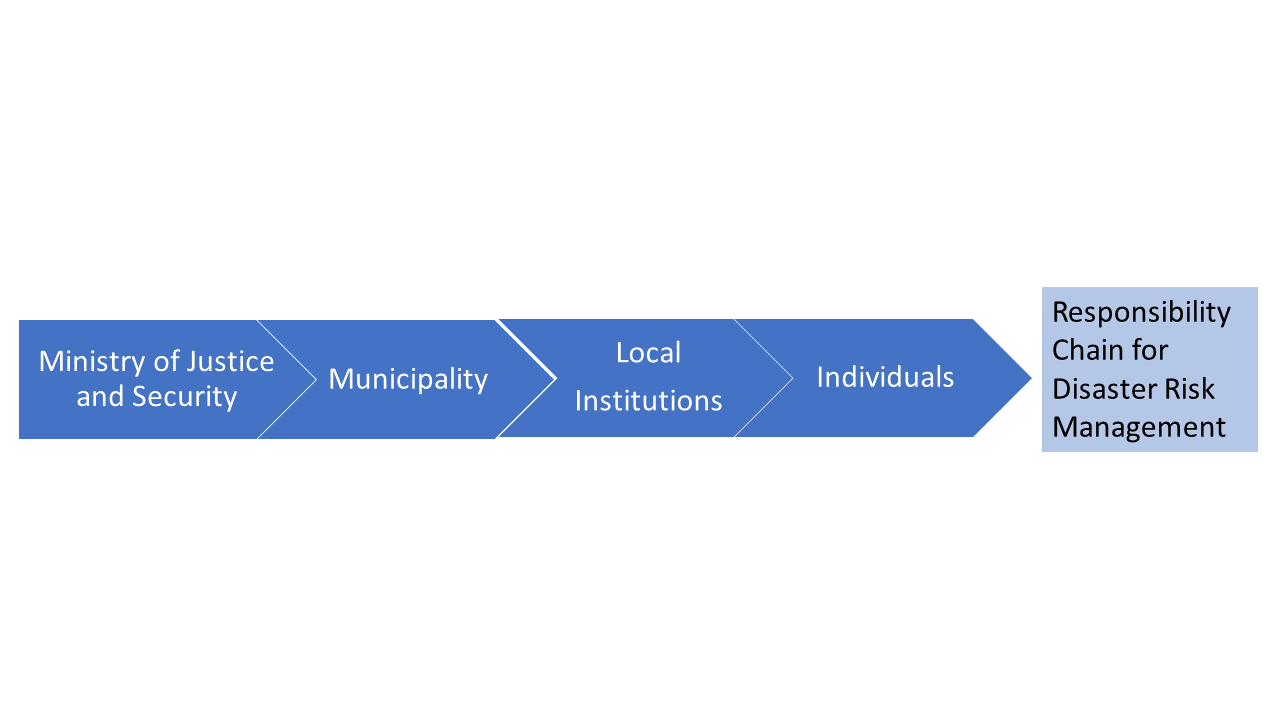
\includegraphics[width=1\textwidth]{fig_theory/responsibility drm.png}
    \caption{Responsibility Hierarchy for Disaster Risk Management in Norway}{ drawing from \cite{rasanen_conceptualizing_2020} and \cite{hanssen_saksframlegg_2013}. The ministry of Justice and Security has the overall responsibility for disaster risk management in Norway. This ministry issues responsibility to the Municipality, which in turn issues responsibility for preparation of disasters to both local institutions and individuals. }
    \label{fig:drm_responsibility}
\end{figure}
\paragraph{}
The overarching responsibility is that of the Ministry of Justice and Security. Responsibility is then transferred to the local municipalities, for the research sites considered here this is the Trondheim Kommune. In turn, while maintaining overall responsibility for disaster risk management, the municipality issues certain tasks to local institutions (\cite{hanssen_saksframlegg_2013}). Certain responsibilities are also issued to the individuals who reside or visit the municipality. This responsibility is communicated in various ways and often by the local institutions. 





\subsection{Natural Systems and Technological Systems impacting Resilience }
Sea levels are discussed in reference to NN2000, Norway's national vertical reference frame. Sea Level extreme (SLE) is the extreme to which the sea reaches in height and area (\cite{nilsen_sealevelchangefornorway_nodate}; \cite{kartverket_se_2020}). The most common sea level extreme is the spring tide. SLEs in Trondheim are the combination of the impact of vertical land movements and the height of the sea, which varies with the tidal cycle, storm surges, winds, and waves \cite{hanssen-bauer_climate_2017} (figure ~\ref{fig:theory_SLE_cause}). The River (Nidelva, figure ~\ref{fig:research_site}), which flows into Trondheimsfjord in the study area can also impact local SLEs during floods and higher flows in spring, for example. Storm surges are difficult to predict (\cite{nilsen_sealevelchangefornorway_nodate}), as are wind patterns (\cite{rod_three_2015}), and storm surges and the SLEs they produce are dependent on the wind. Storm surges - called stromflo in Norwegian -  occur due to the weather conditions, including strong onshore winds and low air pressure (\cite{hanssen_saksframlegg_2013}). 

\paragraph{}

Reference will be made to the 20 year storm surge throughout this thesis, which is the projected recurrence interval of a storm surge of a particular height.  The 20 year storm surge has a 5 percent chance of occurrence each year as this storm surge on average occurs once every 20 years (\cite{hanssen_saksframlegg_2013}). However, with climate change, the recurrence interval of the 20-year storm surge is likely to increase; one of the major impacts of climate change, known as global weirding, where rare events occur more frequently (\cite{wilson_notitle_2019}. The calculations for SLEs in this report utilise the IPCC's fifth assessment report emission scenario RCP 8.5, which is the emission projection for business as usual (\cite{hanssen-bauer_climate_2017}), to avoid underestimating vulnerability and overestimating resilience.  



\begin{figure}[h!]
    \centering
    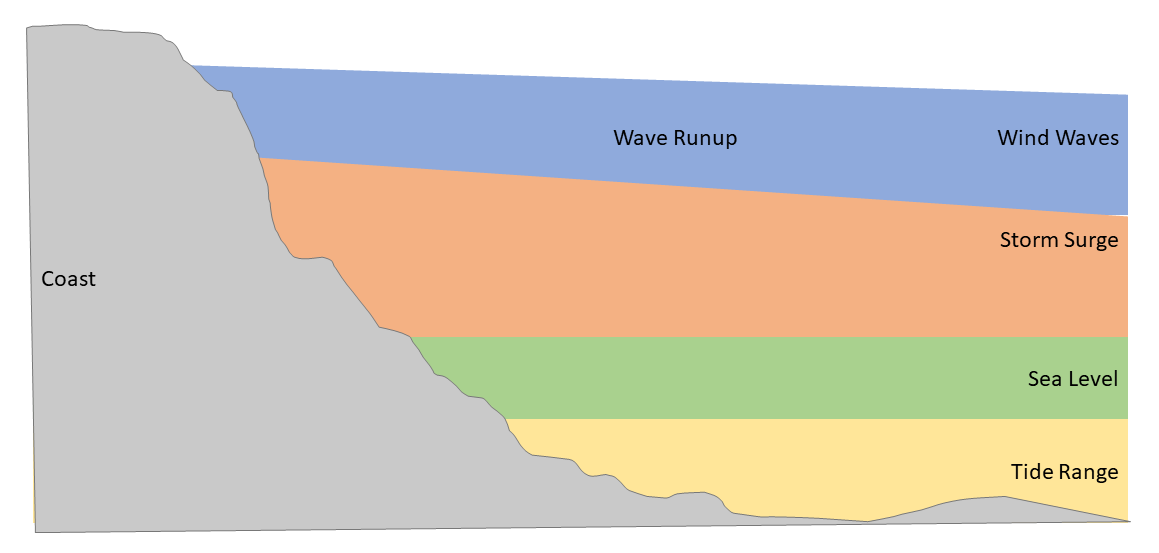
\includegraphics[width=1\textwidth]{fig_theory/sea level extremes.png}
    \caption{The various aspects which combine to create extreme sea levels: Tide Range, Sea Level, Storm Surge, Waves due to the wind, Waves due to the run-up onto the coast.}

    \label{fig:theory_SLE_cause}
\end{figure}

Figure ~\ref{fig:theory_SLE_cause} shows the natural aspects which combine to create SLEs. Which factor is most important will be different for each location, however for all research sites in Trondheim, the largest change between 2022 and 2100 is the projected risk of storm surges. The impact due to waves which may change with the changing climate is predicted to cap out at 2m within the same time frame \cite{hanssen_saksframlegg_2013}. The Safety class 1 of the building regulations TEK10/TEK17 as used since 2016, corresponds with the 20 year storm surge (\cite{tides_high_2022}). The temporal variability and land use characteristics could be considered in an analysis of Trondheim's natural systems resilience to storm surges. However, these factors appear to have minimal impact in urban and semi-urban environments (\cite{hoffken_effects_2020}). For this reason, it is considered as a technological system resilience. Other factors contributing towards technological system resilience includes the artificial altering of the coastlines, the monitoring of the coastlines and general infrastructure beyond buildings.

\section{Theories of Resilience }

There are many theories of resilience and the term has many varied and wide conceptualisations. \cite{moser_turbulent_2019} highlights the recent increase in this term and discusses how different fields use the term resilience.  The increase of the use in response to tragedy, especially tragedy associated with large uncontained systems, is also highlighted. The climate is one such system and the political difficulty of discussing the climate crisis has led many politicians to instead focus on resilience building. 
\paragraph{}

Thus the term resilience is broadened to include a normative and trans-formative aspect.  This moves resilience away from a value that can be measured once, into a ongoing process which increases and decreases over time. The path of this needs to be understood, to prove increases in resilience as required by United Nations Sustainable Development Goals (UN SDGs) 11 and 13. Building resilience is often assumed to always be a desired outcome and is often raised in the response to disaster and especially tragedy (\cite{moser_turbulent_2019}). This newer conceptualisation of resilience allows for greater focus on the integration of local knowledge, but this facet is not always included (\cite{moser_turbulent_2019}).
\paragraph{}


\cite{cutter_place-based_2008} introduced the Determination of Resilience of Place. This was based on previous work on vulnerability and hazards of place (\cite{cutter_vulnerability_1996}).  Vulnerability was labelled as the inherent qualities of the systems which create the potential for harm.
In contrast, in the 2008 work, resilience was the ability to respond and recover which was inherently place based. However, \cite{cutter_community_2020} moved away from place based resilience to focus on community resilience. Now, resilience was considered as dynamic and dependent on three changing systems: natural, social and technological. Present resilience does not define future resilience, but it does influence it. So resilience, be it place based or community resilience, can only be measured post disaster. Both of these understandings of resilience are deemed vital to an overall view of resilience.
\paragraph{}

However, \cite{rasanen_conceptualizing_2020} shows the limitations of a place-based metric for measuring community resilience. They highlight the need for an alternative metric which can include community resilience and local knowledge and which can be repeatedly measured and viewed from a place-based conception of resilience. This is especially vital, as in Norway, the most common conceptualisation of community within national government, municipalities and individuals is place-based (\cite{rasanen_conceptualizing_2020}). To resolve this issue, the concept of projected resilience of place is put forward. 




\section{Projected Resilience of Place} 
\label{theory-resilience}
Resilience is here considered as the ability to return to normality as quickly as possible after an event (\cite{cutter_place-based_2008}). Resilience is dynamic and the current levels of resilience do not define future resilience, but has significant influence. Hence, understanding of current systems which create resilience and how they are changing can let us project resilience (\cite{cutter_community_2020}). The view of resilience here incorporates many of \cite{moser_turbulent_2019} ideas about resilience -  that it can be a system trait, an outcome or a process. It considers projected resilience as a projected outcome, which is determined from systems. 

\begin{figure}[!ht]
    \centering
    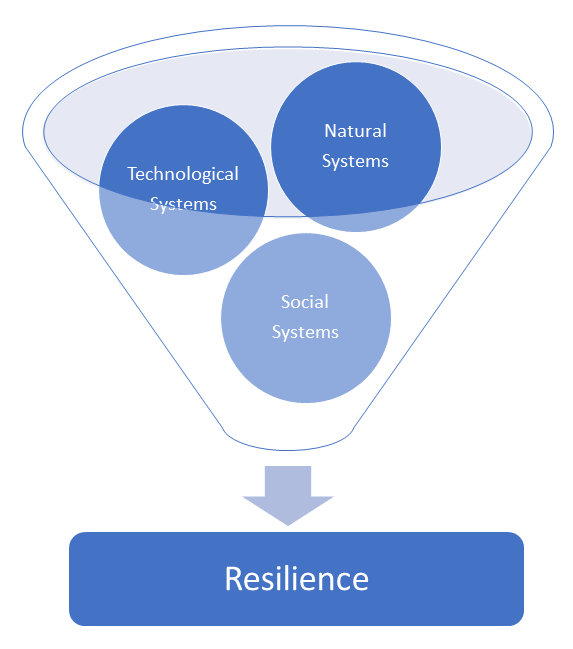
\includegraphics[width=0.5\textwidth]{fig_theory/resilience model .png}
    \caption{Model of Projected Resilience and the systems involved in its creation. The interplay of technological systems, social systems and natural systems creates resilience. }
    \label{fig:projected_resilience}
\end{figure}

\cite{cutter_place-based_2008} and \cite{cutter_community_2020} discuss resilience in reference to disasters rather than events. Moving from measuring resilience post a disaster to projected resilience requires a consideration of the word disaster. SLEs can cause disaster, but this is not necessarily the case. A sea level extreme thus can be viewed as a possible disaster which is referred to here as an event. 
\paragraph{}
An event is a potential disaster in which systems can absorb the impacts in such a manner that normality is not lost. In terms of SLEs, the daily tide flow is not a disaster as it in absorbed by the systems which cope, preventing this event from becoming a disaster. The sensitivity of the system is very rarely breached by the high tide in Trondheim, to date. This distinction of events and disasters may be obvious for events which occur twice a day, but as extreme weather events become the norm, due to the changing climate, what was once a potential disaster if managed will now simply be an event. 
\paragraph{}

Projected resilience takes on the systems as laid out by \cite{cutter_community_2020}, but places community resilience under social systems. This allows for greater understanding between academic, policy makers and "layperson" due to the standard conceptualisation of community as placed based, in Norway as highlighted by \cite{rasanen_conceptualizing_2020}. This is also to allow for an easier determination of resilience so it can be repeatedly measured, without losing the aspects of community resilience or local knowledge. This risk is highlighted by \cite{rasanen_conceptualizing_2020}. The three systems of resilience as shown in figure ~\ref{fig:projected_resilience} are discussed individually in the sections below.



\section{Sustainability vs Resilience}

Sustainability is a term with increasing use and interest over the last decades. There are many similarities between this concept and the concept of resilience. However, the dynamism of the term resilience and its lack of solidified political meaning is often favoured, particularly with groups self-excluded from discussions on sustainability (\cite{moser_turbulent_2019}). This politicisation of the term has benefits and negatives, but risks changing the meaning.
\paragraph{}

While \cite{moser_turbulent_2019} highlights the increasing use of the term resilience to mean an organizing strategy for handling complex systems with high levels of uncertainty, especially in political spheres, this understanding of resilience did not seem the most appropriate for SLEs in Trondheim. In part, because of the high levels of acceptability of the climate crisis both in the local population and in the political spheres, locally, regionally and nationally. Within the political context of Trondheim, neither climate change nor sustainability are excluded terms. Keeping these terms distinct from resilience, allows for a more nuanced discussion.







